\documentclass[preprint,12pt]{elsarticle}
\usepackage[utf8]{inputenc}
\usepackage[T1]{fontenc}
\usepackage{lmodern}
\usepackage{amsmath,amssymb,amsfonts}
\usepackage{graphicx}
\usepackage{booktabs}
\usepackage{longtable}
\usepackage{array}
\usepackage{geometry}
\usepackage{url}
\usepackage{hyperref}
\usepackage{float}
\usepackage{placeins}
\geometry{margin=1in}
\graphicspath{{paper/}{paper/figures/}{figures/}}
\hypersetup{colorlinks=true,linkcolor=black,citecolor=blue,urlcolor=blue,hypertexnames=false}
\urlstyle{same}
\setlength{\emergencystretch}{2em}
\makeatletter
\pdfstringdefDisableCommands{\def\corref#1{}\def\@corref#1{}\def\cnotenum#1{}}
\makeatother
\journal{Journal of Computational Science}
\makeatletter
\long\def\pprintMaketitle{\clearpage
  \iflongmktitle\if@twocolumn\let\columnwidth=\textwidth\fi\fi
  \resetTitleCounters
  \def\baselinestretch{1}%
  \printFirstPageNotes
  \begin{\elsarticletitlealign}%
 \thispagestyle{pprintTitle}%
   \def\baselinestretch{1}%
    \Large\@title\par\vskip18pt%
    \ifx\@elsarticlenewpageafter\newpage@after@title%
      \newpage
    \fi%
    \ifdoubleblind
      \vspace*{2pc}
    \else
      \normalsize\elsauthors\par\vskip10pt
      \footnotesize\itshape\elsaddress\par\vskip36pt
    \fi
    \ifx\@elsarticlenewpageafter\newpage@after@author%
      \newpage
    \fi%
    \ifvoid\absbox\else\unvbox\absbox\par\vskip10pt\fi
    \ifvoid\keybox\else\unvbox\keybox\par\vskip10pt\fi
    \ifx\@elsarticlenewpageafter\newpage@after@abstract%
      \newpage
    \fi%
    \end{\elsarticletitlealign}%
    \gdef\thefootnote{\arabic{footnote}}%
  }
\long\def\MaketitleBox{%
  \resetTitleCounters
  \def\baselinestretch{1}%
  \begin{\elsarticletitlealign}%
   \def\baselinestretch{1}%
    \Large\@title\par\vskip18pt
  \ifdoubleblind
    \vspace*{2pc}
  \else
    \normalsize\elsauthors\par\vskip10pt
    \footnotesize\itshape\elsaddress\par\vskip36pt
  \fi
    \ifvoid\absbox\else\unvbox\absbox\par\vskip10pt\fi
    \ifvoid\keybox\else\unvbox\keybox\par\vskip10pt\fi
    \end{\elsarticletitlealign}%
}
\makeatother

\begin{document}
\begin{frontmatter}
\title{A Model-Conditioned Preflight Protocol for Prior Selection in Node-Wise Scientific Latent Dynamics}
\author[inst1]{Ruiqi Wang\corref{cor1}}
\ead{riw010@ucsd.edu}
\address[inst1]{Department of Physics, University of California San Diego, La Jolla, CA, United States}
\cortext[cor1]{Corresponding author: Ruiqi Wang}
\begin{abstract}

Graph-prior gains in scientific latent dynamics are often reported as
prediction improvements, but such gains do not by themselves show that
the model used the candidate graph topology. We propose a
model-conditioned preflight protocol that decomposes graph-prior
efficacy into three operational attribution classes: (i)
topology-aligned support, requiring agreement between rollout
point-estimate ordering and audit-mode latent-metric separation
against the spectrum-matched permuted graph (SMPG) control;
(ii) generic regularization, where graph priors improve over
no-prior training but the gains do not survive SMPG controls; and
(iii) no effect. Applied across seven regimes including HO lattices,
N-body distance graphs at three connectivities, real-world traffic
(METR-LA), graph-heat and graph-wave lattices, spring-mass systems,
and five rMD17 molecules---totaling 13 measurement cells---the
protocol identifies one controlled audit-positive (topology-aligned
support) case (the HO audit), eight generic-regularization cells
spanning both
N-body synthetic data and real rMD17 molecular-dynamics data, and four
no-effect cells. Across the eight generic-regularization cells, effect
sizes against the no-prior baseline range from 2.4 to 8.4, while effect
sizes against the SMPG control range from (-2.9) to 0.9 with
confidence-interval overlap in every cell. Thus, graph-vs-none
improvements in our evidence would have been over-attributed without
SMPG controls. The protocol is offered as a practical preflight
workflow for prior selection and interpretation under a fixed model
condition; it is not a new graph prior, a universal physics predictor,
a causal discovery method, or a state-of-the-art benchmark.

\end{abstract}
\end{frontmatter}

\section{Introduction}

Scientific dynamics models increasingly combine learned latent-state evolution with auxiliary priors motivated by domain structure. In molecular dynamics, coupled oscillator systems, particle simulations, traffic networks, and graph-discretized physical fields, observations can often be written as trajectories $X_t$ over $N$ interacting nodes. Before fitting a full model, a practitioner may already have a plausible candidate graph, a temporal smoothness assumption, or another regularizer that appears scientifically reasonable. Such priors are attractive because they may stabilize long-horizon rollout prediction, improve sample efficiency, and encode structure that is difficult to infer from limited data alone. Their practical value, however, is not intrinsic to the prior alone. It depends on how the prior interacts with the encoder, transition model, latent dimension, prior placement, optimization setting, training budget, and rollout horizon.

In the settings tested here, this dependence makes graph-prior effects difficult to interpret. A Laplacian penalty on learned node-wise latents may improve rollout because the candidate graph captures meaningful physical or scientific structure. The same gain may also arise because the penalty imposes generic graph-frequency smoothing, because a spectrum-matched permuted graph control would have produced a similar effect, because calibrated temporal smoothing would have been sufficient, or because the apparent advantage is confined to a short budget before an unconstrained model catches up. A graph-aware encoder or transition model can further blur the interpretation by already encoding part of the relational bias. Consequently, in our evidence and protocol, a graph prior outperforming the no-prior baseline establishes practical utility but does not by itself establish topology-specific attribution.

From a computational-science perspective, this ambiguity is costly. In our workflow, sweeps over priors, graph constructions, regularization strengths, seeds, and budgets can still leave attribution unresolved if the comparison set is incomplete. What is often needed first is a smaller decision stage: should the candidate graph be carried into a larger run, should a cheaper graph-free alternative be preferred, or should stronger controls be introduced before any topology-specific attribution claim is made? We therefore frame prior choice as a preflight problem. Before committing to full-scale training, a structured low-cost screen should determine whether a prior is useful, what explains the gain, and what evidence would still be required for stronger interpretation.

This article develops that idea as a model-conditioned preflight protocol for prior selection in node-wise scientific latent dynamics. The protocol compares no-prior training, a candidate graph prior, a spectrum-matched permuted graph control, optional random-graph controls, and calibrated temporal smoothing. Audit mode, used when checkpointed latent traces are available, additionally examines whether predictive gains coincide with latent behavior aligned with the candidate graph. The contribution is methodological rather than architectural: the paper introduces a control-oriented workflow for prior selection and topology-specific attribution, and it uses a conservative label set to convert ambiguous prior effects into an actionable prior recommendation under a specified model condition. The manuscript does not introduce a new graph prior, claim universal physics prediction, frame the task as causal discovery, or present a state-of-the-art benchmark.

\section{Related Work}

This manuscript sits at the intersection of several active lines of research while remaining narrower in scope than any one of them. A first strand comes from geometric deep learning, where graph neural networks, graph-spectral constructions, and graph-based regularizers are used to encode relational inductive bias on non-Euclidean domains \citep{bronstein2021geometric,chung1997spectral}. Prior literature establishes graph structure as useful for prediction and representation learning; our narrower question is attribution under a fixed tested protocol. This paper instead asks: under a fixed latent dynamics model, when does a candidate graph prior merit further computation, and what controls are required before topology-specific attribution is justified?

A second strand concerns scientific and physical latent dynamics models, including world-model formulations that learn compact state representations and transition operators for dynamical systems \citep{hansen2024tdmpc2,hafner2023dreamerv3,hansen2024puppeteer}. In these settings, priors are often introduced to stabilize rollout, improve sample efficiency, or encode known structure suggested by measurement geometry or domain knowledge. The contribution here is complementary rather than competing. The paper does not propose a universal scientific world model; it proposes a standardized, low-cost preflight workflow for deciding whether a candidate prior should be carried into larger runs under a specified model condition.

A third strand includes causal and structural representation learning \citep{scholkopf2021toward}. That literature seeks latent variables or relational structure aligned with underlying mechanisms, and it often asks whether learned representations capture more than predictive convenience. The present manuscript adopts some of the same caution about interpretation, but its goal is narrower. The workflow compares predictive priors under matched controls and asks whether observed gains support topology-specific attribution. It is not a causal discovery method, and it does not attempt to identify a true interaction graph from data alone.

A fourth strand concerns model-selection, ablation, and diagnostic workflows in machine learning and computational science. These approaches emphasize controlled baselines, matched comparisons, calibration, ablation, and concise reporting to guide computational decisions. The present protocol belongs most directly in this tradition. Its emphasis is on matched prior comparisons, persistence checks, and optional audits that produce an actionable prior recommendation before larger sweeps are undertaken, rather than on claiming state-of-the-art benchmark performance.

Taken together, these literatures motivate the need for the present study while also clarifying its boundary. This paper should be read as a prior-selection and attribution workflow for node-wise scientific latent dynamics: it draws on graph-based inductive bias, latent dynamics modeling, and diagnostic practice, but it does not claim a new graph architecture, a causal discovery result, or a state-of-the-art benchmark.

\section{Problem formulation}

We consider node-wise physical or scientific trajectory data $X_{1:T}$, where each frame $X_t \in \mathbb{R}^{N\times d}$ contains $d$ observed features for each of $N$ nodes. A dataset adapter provides these trajectories, a candidate graph or graph Laplacian $L \in \mathbb{R}^{N\times N}$, and metadata describing the graph source, the underlying simulator or dataset, and whether the graph is known, approximate, constructed, or data-derived. The predictive model maps observations into learned latent node states $H_t \in \mathbb{R}^{N\times m}$ and trains a transition model to forecast future dynamics.

The relevant object for interpretation is the model condition. In this manuscript, the model condition comprises the encoder, transition model, latent dimension, prior placement, optimizer settings, prior strength, training budget, and rollout evaluation horizon. A preflight result is therefore not a dataset-level truth statement. It is a recommendation tied to the tested model condition and must be reconsidered if the architecture, prior location, regularization strength, budget, or evaluation horizon changes.

The central question is the following:

\begin{quote}
Under this model condition and training budget, does a candidate prior improve rollout prediction, and is the improvement better attributed to candidate topology, generic graph-frequency smoothing, calibrated temporal smoothing, or a low-budget regularization effect?
\end{quote}

This formulation is intentionally narrower than causal discovery, universal physics modeling, or benchmark optimization. The objective is to reduce unnecessary full-training compute, avoid false topology-specific attribution, and decide whether the next step should be no prior, a candidate graph prior, calibrated temporal smoothing, or audit mode. Throughout the reported experiments, rollout quality is summarized at fixed horizons, especially $H=16$ and $H=32$, with $H=32$ serving as the principal manuscript readout.

Two non-goals follow directly from this framing. First, the protocol does not claim that a useful candidate graph is physically true. Second, it does not claim universal coverage across scientific systems. The experiments are therefore presented as representative node-wise physical/scientific dynamics regimes rather than as a universal physics prediction study.

\section{Mathematical and computational framing}

The protocol separates prior utility from topology-specific attribution by evaluating several prior families under the same model condition, with the graph-spectral viewpoint following standard references in spectral graph theory \citep{chung1997spectral}. The baseline condition is \texttt{none}, in which the latent dynamics model is trained without an auxiliary prior. The principal candidate graph prior is graph Laplacian smoothness on learned node-wise latent states. For a latent matrix $H$, the graph penalty is

\begin{equation}
R_G(H;L)=\mathrm{Tr}(H^\top L H)
\end{equation}

If $L = U \Lambda U^\top$ is the eigendecomposition of the Laplacian and $H = U A$, then

\begin{equation}
\mathrm{Tr}(H^\top L H)=\mathrm{Tr}(A^\top \Lambda A)=\sum_k \lambda_k \lVert a_k \rVert_2^2
\end{equation}

This identity clarifies why graph-prior gains require caution. The candidate graph prior penalizes high graph frequencies more strongly, so improved rollout may reflect useful scientific structure, but it may also reflect generic smoothing in the graph spectral domain.

To probe that distinction, the key attribution baseline is the spectrum-matched permuted graph control. With permutation matrix $P$, the control Laplacian is

\begin{equation}
L_{\mathrm{perm}}=P^\top L P
\end{equation}

This transformation preserves the eigenvalues of $L$, and hence the scale of graph-frequency smoothing, while disrupting node-label semantics. Within this protocol, if the candidate graph prior improves over the no-prior baseline but not over the spectrum-matched permuted graph control, the evidence supports predictive smoothing rather than topology-specific attribution. Random-graph controls can be informative secondary checks, but they are weaker because they do not preserve the full Laplacian spectrum.

The protocol also includes a graph-free baseline,

\begin{equation}
R_T(H_{1:T})=\sum_t \lVert H_{t+1}-H_t \rVert_F^2
\end{equation}

which we refer to as calibrated temporal smoothing when its effective regularization scale has been matched to the candidate graph prior. Calibration is necessary because raw temporal losses can be much smaller than graph-Laplacian losses. If $\alpha_G$ denotes the graph-prior weight and $R_G^0$ and $R_T^0$ denote initial auxiliary-loss values measured under the same calibration pass, the temporal weight is chosen as

\begin{equation}
\alpha_T = \frac{\alpha_G R_G^0}{R_T^0+\varepsilon}
\end{equation}

so that

\begin{equation}
\alpha_T R_T^0 \approx \alpha_G R_G^0
\end{equation}

This calibration does not assert that graph and temporal priors are equivalent. It ensures that the comparison asks a fairer question: at matched initial regularization strength, does the candidate graph add value beyond graph-free temporal smoothing? The same framing also clarifies why, in our evidence, graph versus none alone is insufficient for topology-specific attribution. That stronger interpretation requires explicit comparison with the spectrum-matched permuted graph control and with calibrated temporal smoothing.

\section{Model-conditioned preflight protocol}
\label{sec:protocol}

The model-conditioned preflight protocol is designed as a staged computational screen rather than a substitute for full training. It begins with diagnostics that summarize the candidate graph and the observed dynamics, proceeds to controlled mini-training runs, and escalates to longer budgets or latent audits only when the quick result warrants additional analysis.

Operationally, the workflow has four stages. First, trajectories, candidate graph metadata, and the corresponding Laplacian are loaded from a dataset adapter. Second, the prior family set is defined: \texttt{none}, the candidate graph prior, the spectrum-matched permuted graph control, optional random-graph controls, and calibrated temporal smoothing when a graph-versus-temporal comparison is needed. Third, models are trained under a screening budget and, when justified, under a longer budget; rollout is evaluated at fixed horizons. Fourth, if checkpointed latent traces are available, audit mode examines whether rollout gains coincide with smoother or more low-frequency latent temporal deltas in the candidate graph basis.

Figure 1 summarizes this workflow.

\begin{figure}[!htbp]
\centering
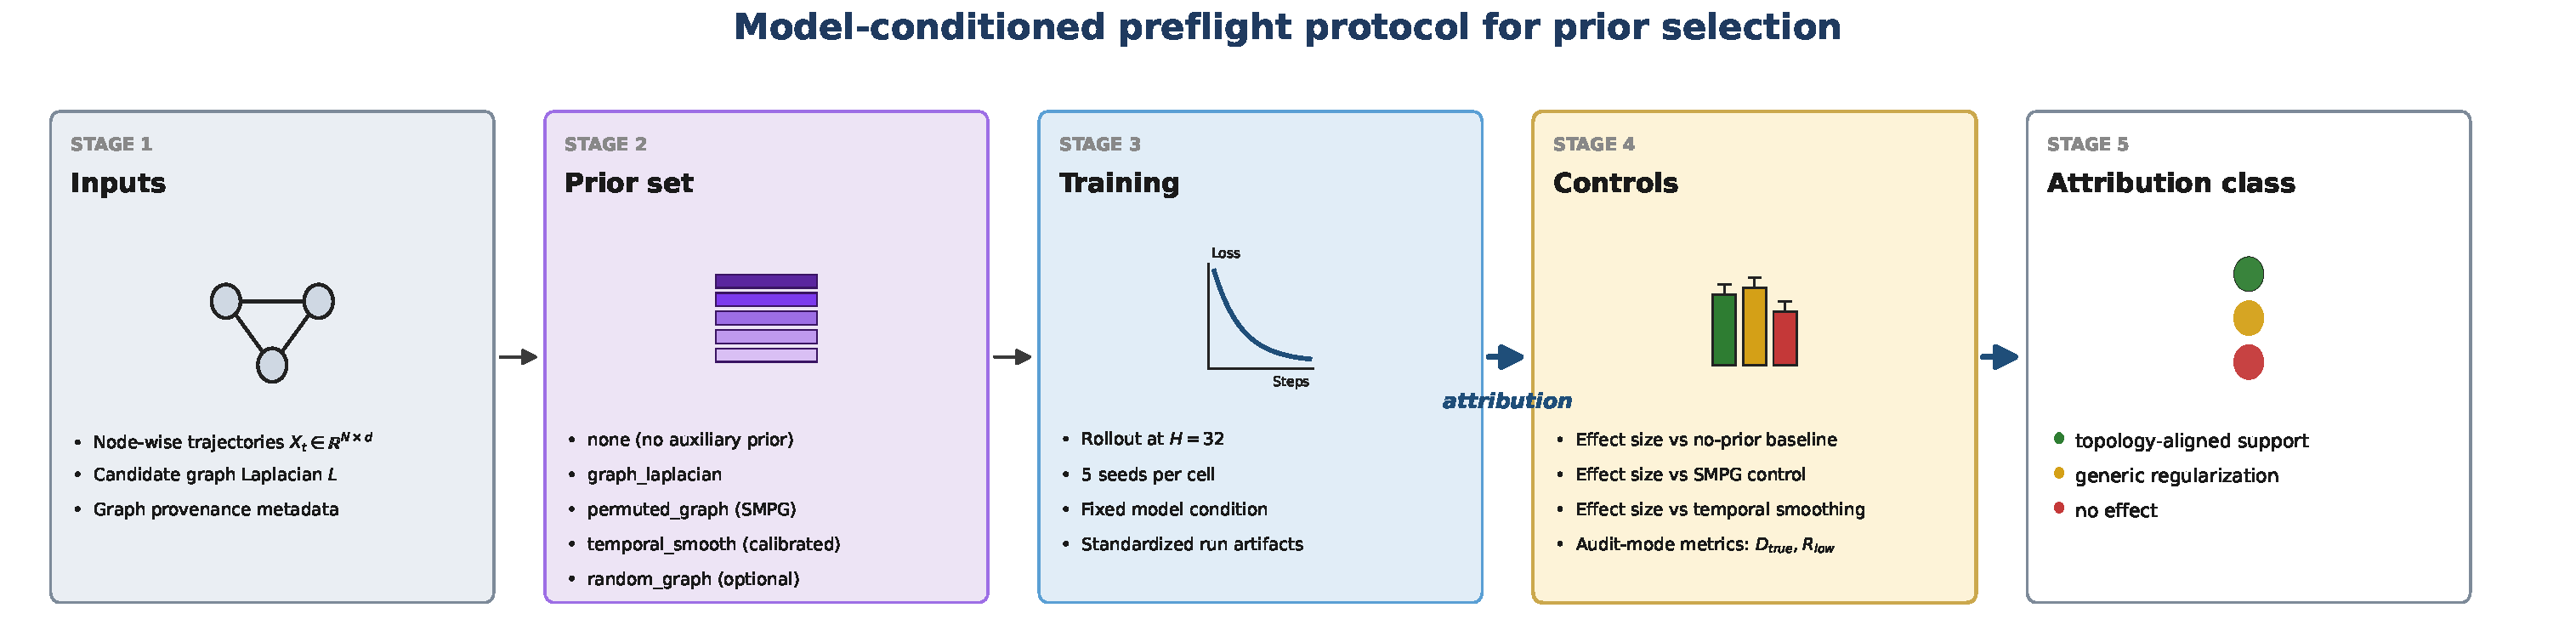
\includegraphics[width=\linewidth]{figures/fig_protocol_overview.pdf}
\caption{Model-conditioned preflight workflow. The protocol converts prior selection into a staged computational decision. Node-wise trajectories and a candidate graph first pass through raw diagnostics, then matched-prior comparisons against the spectrum-matched permuted graph (SMPG) control and calibrated temporal smoothing. An optional audit mode checks whether predictive gains coincide with smoother and more low-frequency learned latent temporal deltas in the candidate-graph basis. The output is an actionable prior recommendation under the tested model condition rather than a claim that the candidate graph is physically true.}
\label{fig:protocol-schematic}
\end{figure}

Audit mode is used when checkpointed latent traces are available; it asks whether predictive gains coincide with latent behavior aligned with the candidate graph and provides the strongest available evidence for topology-aligned support. Figure~\ref{fig:decision-logic} shows how these comparisons lead to topology-specific attribution only when the relevant controls have been cleared.

\begin{figure}[!htbp]
\centering
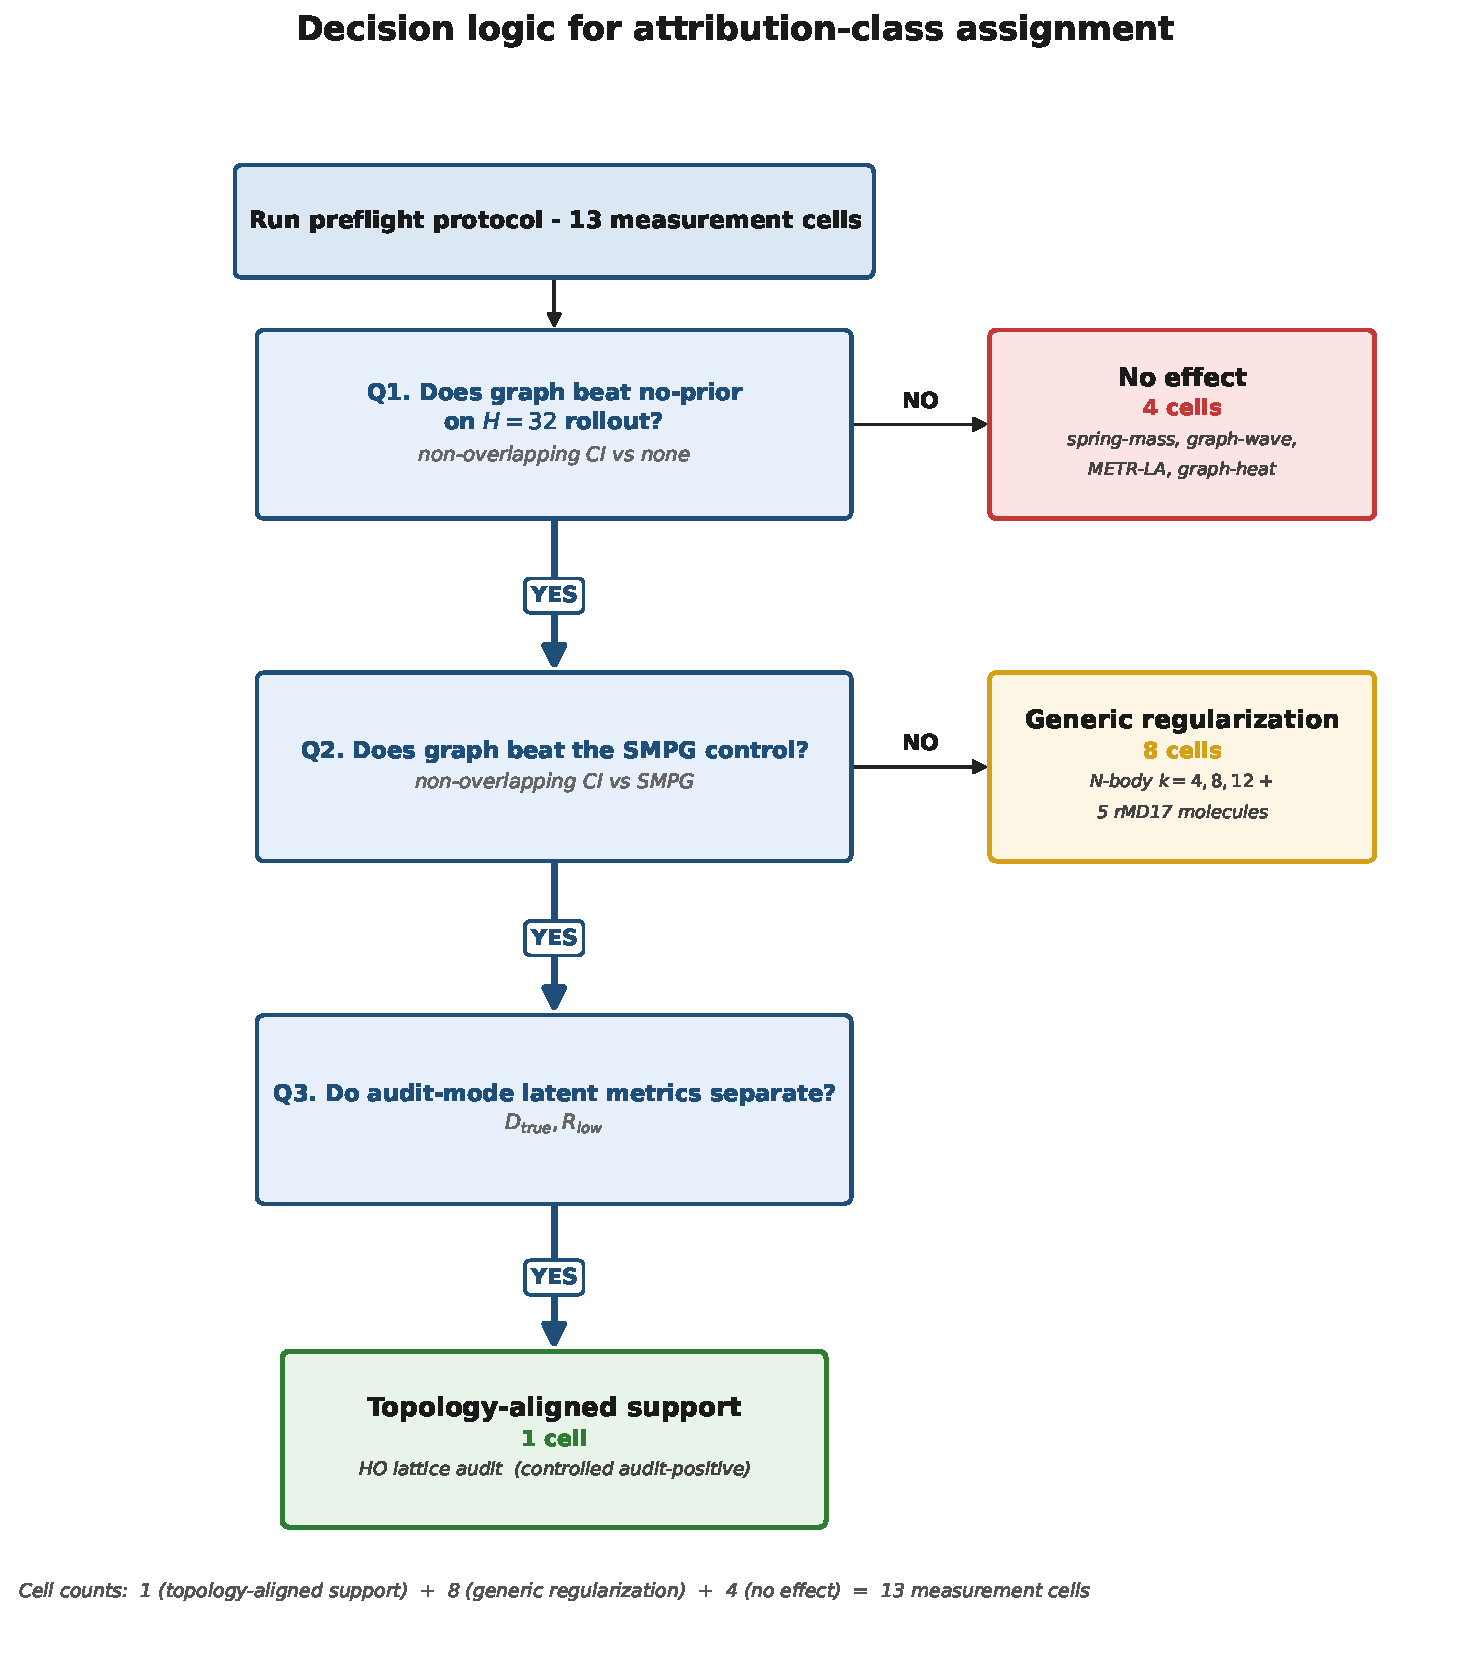
\includegraphics[width=\linewidth]{figures/fig_decision_tree.pdf}
\caption{Decision logic for attribution-class assignment. The decision tree separates predictive utility from topology-specific attribution. A candidate graph must first improve over no-prior training, then beat the spectrum-matched permuted graph (SMPG) control under the operational non-overlapping confidence-interval criterion before it supports topology-specific attribution under the tested condition. Audit-mode latent metrics, when available, provide the strongest evidence of topology-aligned support. Cells that improve over no-prior but do not separate from SMPG are classified as generic regularization; cells that fail to improve over no-prior are classified as no-effect.}
\label{fig:decision-logic}
\end{figure}

The resulting labels are listed in Table 1, and the prior families on which they depend are summarized in Table 2. Taken together, these tables define the vocabulary of the protocol and the corresponding actionable prior recommendation associated with each outcome.

\begingroup
\scriptsize
\setlength{\tabcolsep}{3pt}
\renewcommand{\arraystretch}{1.08}
\begin{longtable}{>{\raggedright\arraybackslash}p{0.15\textwidth}>{\raggedright\arraybackslash}p{0.22\textwidth}>{\raggedright\arraybackslash}p{0.21\textwidth}>{\raggedright\arraybackslash}p{0.15\textwidth}>{\raggedright\arraybackslash}p{0.19\textwidth}}
\caption{Protocol labels and corresponding actionable prior recommendations}\label{tab:protocol-labels}\\
\toprule
\textbf{display label} & \textbf{evidence pattern} & \textbf{recommended action} & \textbf{claim allowed} & \textbf{claim boundary} \\
\midrule
\endfirsthead
\toprule
\textbf{display label} & \textbf{evidence pattern} & \textbf{recommended action} & \textbf{claim allowed} & \textbf{claim boundary} \\
\midrule
\endhead
\midrule
\multicolumn{5}{r}{\emph{Continued on next page}} \\
\midrule
\endfoot
\bottomrule
\endlastfoot
no prior gain & No tested prior improves meaningfully over the no-prior model. & Skip the prior for larger runs unless there is a separate scientific reason to test it. & The tested prior was not useful under the model condition. & Does not imply the prior is useless for all models or budgets. \\
generic smoothing & The candidate graph improves over no-prior training but does not beat the spectrum-matched permuted graph control or comparable smoothing controls. & Treat the result as smoothing-like and test cheaper or simpler controls first. & Graph-style regularization helped prediction. & Do not claim topology-specific attribution. \\
temporal sufficient & Calibrated temporal smoothing matches or beats the candidate graph prior. & Prefer calibrated temporal smoothing unless topology-specific attribution is itself the objective. & Graph-free temporal smoothing explains the observed gain. & Do not claim that graph structure is necessary. \\
candidate topology & The candidate graph beats no-prior training, the spectrum-matched permuted graph control, and calibrated temporal smoothing under the tested budget. & Carry the candidate graph forward with more seeds, stronger controls, and audit where possible. & The result supports topology-specific attribution under the tested condition. & It does not prove that the candidate graph is the true physical interaction graph. \\
topology-aligned audit & Rollout gains coincide with smoother or more low-frequency learned latent temporal deltas in the candidate graph basis. & Use as the strongest preflight support for continuing the candidate graph. & Audit evidence supports topology-aligned latent smoothing under the tested condition. & The result remains model-conditioned, weight-conditioned, and budget-conditioned. \\
overconstrained & A prior harms rollout relative to no-prior training and controls. & Reduce strength, revise prior placement, or skip the prior. & The tested prior suppressed useful predictive variation. & This does not rule out weaker or differently placed priors. \\
inconclusive & Required controls, seeds, or audit artifacts are insufficient. & Run the missing controls or avoid stronger claims. & Evidence is insufficient for a stronger label. & Do not over-interpret incomplete comparisons. \\
\end{longtable}
\endgroup

\begingroup
\footnotesize
\setlength{\tabcolsep}{4pt}
\begin{longtable}{>{\raggedright\arraybackslash}p{0.15\textwidth}>{\raggedright\arraybackslash}p{0.29\textwidth}>{\raggedright\arraybackslash}p{0.27\textwidth}>{\raggedright\arraybackslash}p{0.21\textwidth}}
\caption{Prior families and attribution roles}\label{tab:prior-families}\\
\toprule
\textbf{prior family} & \textbf{definition} & \textbf{attribution role} & \textbf{manuscript use} \\
\midrule
\endfirsthead
\toprule
\textbf{prior family} & \textbf{definition} & \textbf{attribution role} & \textbf{manuscript use} \\
\midrule
\endhead
\midrule
\multicolumn{4}{r}{\emph{Continued on next page}} \\
\midrule
\endfoot
\bottomrule
\endlastfoot
\path{none} & No auxiliary prior. & Establishes whether any prior improves rollout. & Baseline for all preflight recommendations. \\
\path{graph_laplacian} & Candidate-graph Laplacian smoothness on learned node-wise latents, $\mathrm{Tr}\left(H^\top L H\right)$. & Tests whether candidate graph-frequency smoothing helps the tested model. & Main prior under evaluation, not introduced as a new prior. \\
\path{permuted_graph} & Spectrum-matched permuted Laplacian, $L_{\mathrm{perm}} = P^\top L P$. & Preserves Laplacian spectrum while removing node-label semantics. & Primary control for topology attribution in this protocol. \\
\path{random_graph} & Optional graph with matched coarse size or edge statistics. & Tests whether an unrelated graph can produce similar smoothing. & Secondary control; weaker than the spectrum-matched permuted graph control. \\
\path{temporal_smooth} & Graph-free smoothness on learned latent temporal deltas, e.g. $\sum_t \lVert H_{t+1}-H_t \rVert_F^2$. & Tests whether temporal regularization explains candidate graph gains. & Must be calibrated when compared with graph priors. \\
future priors & Planned auxiliary baselines for additional scientific structure. & Broadens the preflight family set. & Mentioned as future extensions, not current core evidence. \\
\end{longtable}
\endgroup

\subsection*{Implementation Overview}

In practice, the preflight workflow is executed through an adapter-based preflight script. Each adapter is responsible for dataset-specific trajectory loading and for supplying the candidate graph information needed by the model-conditioned comparison. Depending on the regime, this means either loading a candidate graph Laplacian directly or constructing the candidate graph Laplacian from dataset-specific metadata before the matched prior comparisons are run.

This design keeps the comparison logic uniform across datasets. Once trajectories, the candidate graph Laplacian, and the associated metadata have been exposed through the adapter interface, the same preflight routine can evaluate no-prior training, the candidate graph prior, the spectrum-matched permuted graph control, optional random-graph controls, and calibrated temporal smoothing under a shared model condition. The resulting artifacts are written in a standardized form: \path{run_config.json} records the run specification, \path{summary.csv} provides the compact metric summary, and \path{preflight_report.md} provides the human-readable interpretation and actionable prior recommendation.

The implementation is also intended to make extension straightforward without changing the underlying methodology. New dataset support is added through adapters rather than by rewriting the core preflight procedure, so the same low-cost screening can be applied before larger sweeps, longer budgets, or expanded seed studies. In that sense, the implementation overview is part of the methodological contribution: it operationalizes standardized low-cost screening while keeping dataset-specific loading and candidate graph construction isolated from the matched prior comparisons themselves.

\FloatBarrier

\section{Experimental regimes and implementation}

The experiments are presented as a stress test of the preflight methodology rather than as a leaderboard. All reported values are drawn from existing completed runs and summaries documented in the accompanying source materials; no new experiments are introduced in this revision. The purpose of the experimental section is to ask whether a single model-conditioned protocol can return sensible decisions across representative node-wise physical/scientific dynamics regimes.

The benchmark set spans controlled oscillator lattices, spring-mass systems, graph-wave and graph heat lattices, a graph low-frequency stress test, approximate n-body interactions, molecular dynamics summaries related to MD17/rMD17 \citep{chmiela2017gdml,christensen2020gradients}, and a traffic forecasting case connected to METR-LA as popularized by DCRNN \citep{li2018dcrnn}. These regimes differ not only in the underlying dynamics but also in candidate graph provenance: some graphs are simulator-defined, some are approximate physical constructions, some are synthetic stress tests, and some are data-derived. This heterogeneity is intentional because the provenance of the candidate graph is part of the interpretation boundary.

Implementation settings are fixed within each model condition. The screening budget used here is typically five epochs; longer-budget runs use twenty epochs where available. Audit mode is used only when checkpointed latent traces are available. Rollout comparisons focus on $H=32$, which is the central summary statistic used throughout the figures and tables. Table 3 summarizes the regimes and the role each plays in the manuscript, while detailed file-level traceability is retained in Appendix D.

\begingroup
\footnotesize
\setlength{\tabcolsep}{3pt}
\renewcommand{\arraystretch}{1.06}
\begin{longtable}{>{\raggedright\arraybackslash}p{0.13\textwidth}>{\raggedright\arraybackslash}p{0.17\textwidth}>{\raggedright\arraybackslash}p{0.22\textwidth}>{\raggedright\arraybackslash}p{0.36\textwidth}}
\caption{Benchmark regimes used for preflight stress testing}\label{tab:benchmark-regimes}\\
\toprule
\textbf{regime} & \textbf{graph source} & \textbf{role in manuscript} & \textbf{key preflight readout} \\
\midrule
\endfirsthead
\toprule
\textbf{regime} & \textbf{graph source} & \textbf{role in manuscript} & \textbf{key preflight readout} \\
\midrule
\endhead
\midrule
\multicolumn{4}{r}{\emph{Continued on next page}} \\
\midrule
\endfoot
\bottomrule
\endlastfoot
HO lattice & true lattice & Controlled topology-specific audit-positive case. & The candidate graph improves H32 rollout and the Cycle 8 audit shows smoother, more low-frequency latent deltas on the true graph. \\
Spring-mass lattice & true spring lattice & Second-order mechanics and temporal-baseline check. & The quick candidate graph gain is explained by calibrated temporal smoothing; the standard budget favors no-prior training. \\
Graph-wave lattice & true wave lattice & PDE-like propagation and temporal-baseline check. & The quick candidate graph gain is smoothness-like; calibrated temporal smoothing slightly beats the candidate graph; the standard budget favors no-prior training. \\
N-body distance & initial distance-kNN weighted graph & Approximate long-range interaction graph. & The quick candidate graph beats no-prior training, the spectrum-matched permuted graph control, and calibrated temporal smoothing; the standard budget favors the spectrum-matched permuted graph control. \\
METR-LA correlation graph & data-derived \path{correlation_topk} sensor graph & Real traffic application case. & Raw alignment does not translate into rollout gain; the candidate graph is worse than no-prior training and the spectrum-matched permuted graph control. \\
Graph heat lattice & true generator graph & Cautionary graph-generated case. & The true generator graph does not help the tested latent model; the candidate graph harms H32 rollout. \\
Graph low-frequency lattice & constructed low-frequency Laplacian basis & Synthetic alignment stress test. & Strong raw alignment does not guarantee quick topology-specific attribution; budget dependence appears in follow-up analysis. \\
rMD17 molecular dynamics summaries & molecular cutoff graphs & Earlier graph-style smoothing and specificity stress test. & Graph-style priors improve rollout, but exact molecular topology-specific attribution is weak against controls. \\
\end{longtable}
\endgroup

\section{Results}
\label{sec:results}

We organize results around the three operational attribution classes 
introduced in Section~\ref{sec:protocol}. Across 13 measurement cells 
spanning seven regimes, the protocol identifies one controlled 
audit-positive / topology-aligned support case, eight 
generic-regularization cells, and four no-effect cells. 
Table~\ref{tab:headline} summarizes; the rest of this section walks 
through each class with detailed numbers from 
Table~\ref{tab:effect-size}.

\begin{table}[h]
\centering
\scriptsize
\setlength{\tabcolsep}{3pt}
\caption{Headline attribution table across 13 measurement cells. Classification key: \texttt{controlled\_audit\_positive} denotes the controlled audit-positive / topology-aligned support class (HO audit only); \texttt{generic\_regularization} denotes cells where graph improves over no-prior but does not separate from SMPG control under non-overlapping CI criterion; \texttt{no\_effect} denotes cells with no meaningful candidate-graph effect.}
\label{tab:headline}
\resizebox{\textwidth}{!}{%
\begin{tabular}{llclcc}
\toprule
regime & cell & n\_seeds & classification & effect vs none & effect vs permuted \\
\midrule
\path{ho_audit_5seed} & \path{ho_lattice_audit} & 5 & \texttt{controlled\_audit\_positive} & N/A & $3.083$ \\
\path{nbody_robustness_5seed} & \path{distance_k_04/standard_ep20} & 5 & \texttt{generic\_regularization} & $6.014$ & $0.535$ \\
\path{nbody_robustness_5seed} & \path{distance_k_08/standard_ep20} & 5 & \texttt{generic\_regularization} & $4.768$ & $-0.370$ \\
\path{nbody_robustness_5seed} & \path{distance_k_12/standard_ep20} & 5 & \texttt{generic\_regularization} & $4.824$ & $0.906$ \\
\path{rmd17_cycle2_3seed} & aspirin & 3 & \texttt{generic\_regularization} & $8.367$ & $0.147$ \\
\path{rmd17_cycle2_3seed} & ethanol & 3 & \texttt{generic\_regularization} & $5.196$ & $-2.935$ \\
\path{rmd17_cycle2_3seed} & malonaldehyde & 3 & \texttt{generic\_regularization} & $3.979$ & $-0.445$ \\
\path{rmd17_cycle2_3seed} & naphthalene & 3 & \texttt{generic\_regularization} & $6.785$ & $0.191$ \\
\path{rmd17_cycle2_3seed} & toluene & 3 & \texttt{generic\_regularization} & $2.359$ & $-0.289$ \\
\path{graph_heat_lattice} & \path{legacy_ep5_no_quick_tag} & 1 & \texttt{no\_effect} & N/A & N/A \\
\path{graph_wave_5seed} & \path{standard_ep20} & 5 & \texttt{no\_effect} & $0.352$ & $-0.469$ \\
\path{metr_la_3seed} & \path{corr_T2000_train160_ep5} & 3 & \texttt{no\_effect} & $-0.736$ & $-0.132$ \\
\path{spring_mass_5seed} & \path{standard_ep20} & 5 & \texttt{no\_effect} & $0.088$ & $0.189$ \\
\bottomrule
\end{tabular}
}
\end{table}

\subsection{Controlled audit-positive / topology-aligned support: HO lattice audit}
\label{sec:ho-audit}

The HO lattice audit is the only controlled audit-positive / 
topology-aligned support cell in our evidence. Its rollout point 
estimates favor the candidate graph (H32 = 0.0169 ± 0.0054 versus 
SMPG 0.0198 ± 0.0059 and random 0.0199 ± 0.0062), but the 95\% 
rollout confidence intervals overlap across the three arms (graph 
$[0.0102, 0.0236]$; SMPG $[0.0125, 0.0271]$; random $[0.0122, 
0.0275]$). We therefore do not treat rollout point-estimate ordering 
alone as evidence of topology-aligned support. The stronger evidence 
comes from audit-mode latent metrics, which are separated in the 
expected direction: the candidate-graph latent temporal delta norm 
\(D_{\mathrm{true}}(\Delta H)\) is 2.81 ± 0.04 versus 3.51 ± 0.11 for 
SMPG, and the low-frequency fraction \(R_{\mathrm{low}}\) at K=4 is 
0.187 ± 0.012 versus 0.122 ± 0.009 for SMPG. The agreement between 
rollout point-estimate ordering and latent audit-metric separation 
forms our operational basis for classifying HO as audit-positive. We 
bound this interpretation: it is a controlled audit-positive case in 
a setting where the candidate graph corresponds exactly to the 
physical Laplacian; it is not a topology-discovery result and is not 
evidence that distance-kNN or other approximate graphs in our other 
regimes would behave similarly.

\begin{figure}[h]
\centering
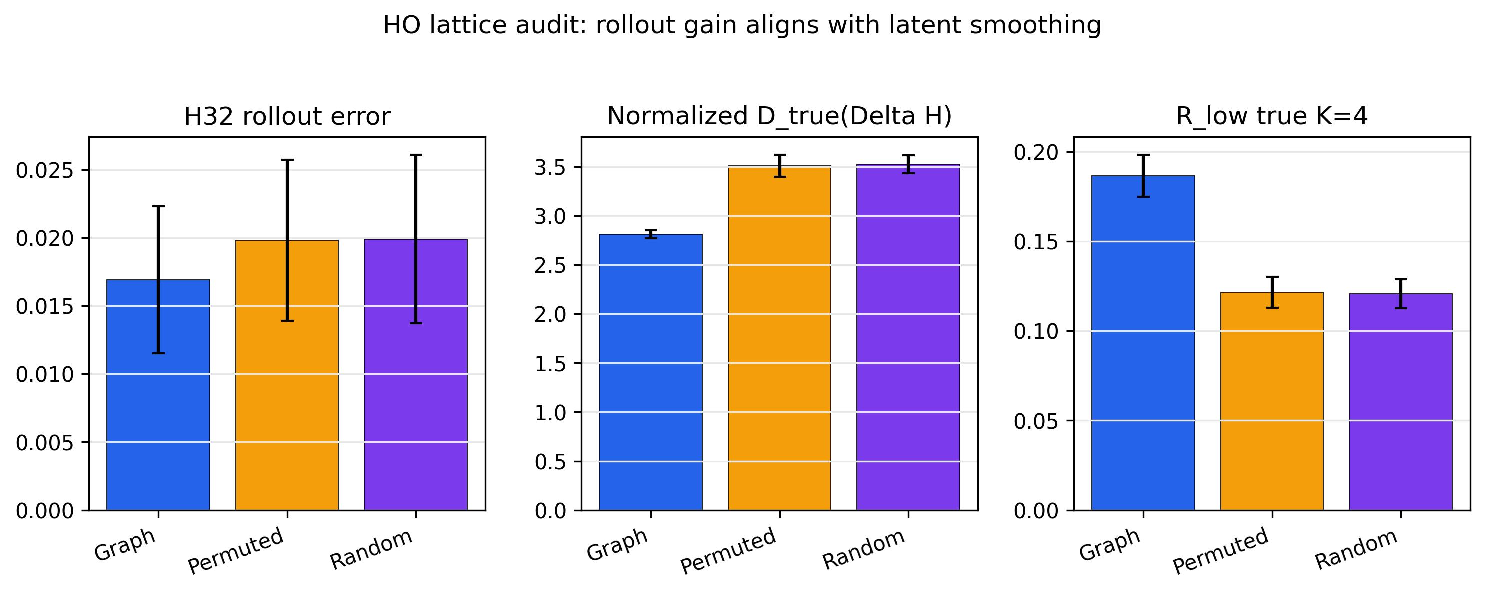
\includegraphics[width=0.85\linewidth]{figures/fig6_latent_audit_positive_case.pdf}
\caption{HO lattice audit: controlled audit-positive case. The 
candidate-graph latent temporal deltas are smoother and more 
low-frequency in the candidate-graph basis than the SMPG and 
random-graph controls. Rollout confidence intervals overlap across 
the three arms; the audit-positive classification rests on the 
agreement between rollout point-estimate ordering and latent 
audit-metric separation.}
\label{fig:ho-audit}
\end{figure}

\subsection{Generic regularization across synthetic and molecular dynamics}
\label{sec:generic-reg}

Eight cells form the generic-regularization block: three N-body 
standard cells at distance-$k$ connectivities $k=4$, $8$, $12$, and 
five rMD17 Cycle-2 molecules.

\paragraph{N-body distance-$k$ standard cells.}
Figure~\ref{fig:nbody-standard} shows the standard-budget rollout for 
the three N-body cells. In all three, the candidate graph substantially 
improves rollout error over no-prior training. At H32, the candidate 
graph achieves 0.064 ± 0.032 ($k$=4), 0.081 ± 0.033 ($k$=8), and 
0.077 ± 0.031 ($k$=12), versus no-prior baselines of 0.151 ± 0.013, 
0.152 ± 0.012, and 0.144 ± 0.012, respectively. Effect sizes against 
the no-prior baseline are 6.01, 4.77, 4.82 with non-overlapping CIs 
in all three cases. Against the SMPG control, however, effect sizes 
fall to 0.54, $-0.37$, 0.91 with confidence-interval overlap in every 
cell, and against calibrated temporal smoothing they fall to 0.14, 
$-0.80$, $-1.27$ with overlap. Under the operational CI criterion, 
the candidate graph is not statistically separable from the SMPG 
control in any of the three connectivities. We therefore attribute 
the graph-vs-none improvement to generic regularization rather than 
to identifiable distance-kNN topology.

\begin{figure}[!htbp]
\centering
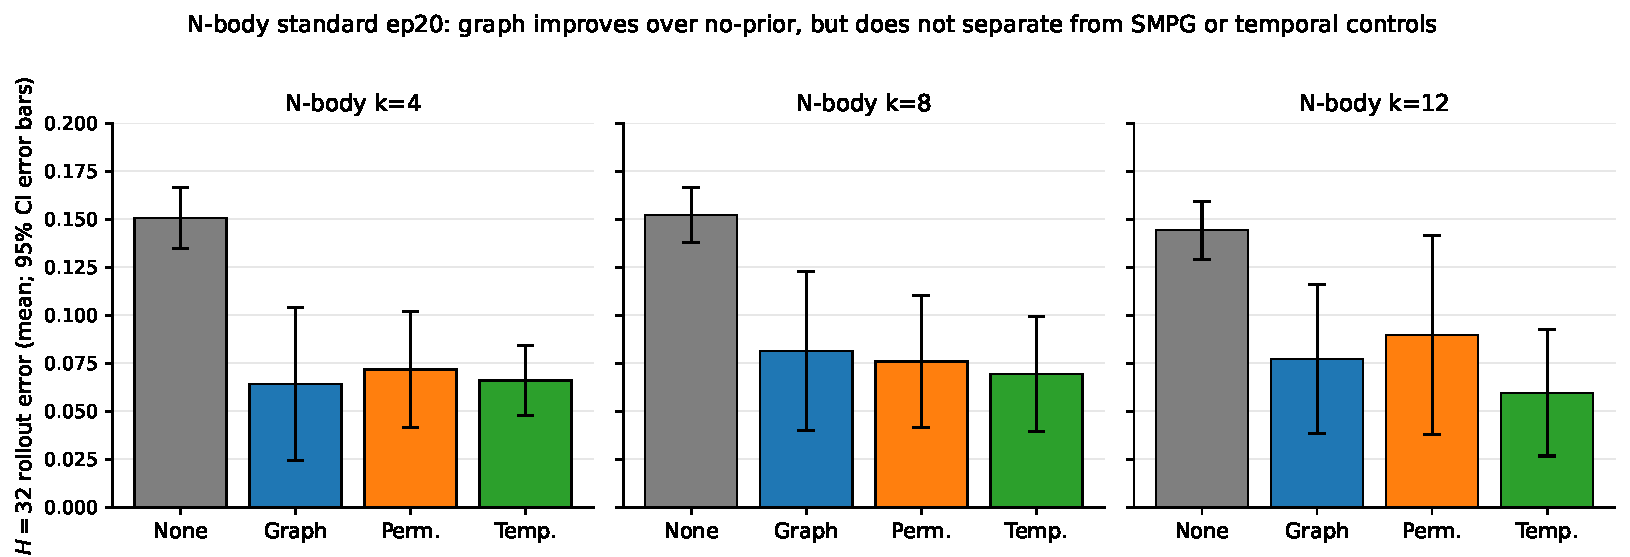
\includegraphics[width=0.95\linewidth]{figures/fig_nbody_standard_3panel.pdf}
\caption{N-body standard-budget rollout (20 epochs, 5 seeds, $H{=}32$). In all three connectivities ($k{=}4, 8, 12$) the candidate distance-kNN graph (Graph) substantially reduces rollout error against the no-prior baseline (None), but the spectrum-matched permuted graph control (Perm.) and calibrated temporal smoothing (Temp.) achieve comparable or slightly better mean rollout. Error bars are 95\% confidence intervals (t-distribution, df=4). Under the operational non-overlapping CI criterion, the candidate graph is not statistically separable from either control in any of the three cells.}
\label{fig:nbody-standard}
\end{figure}

\paragraph{rMD17 molecular-dynamics cells.}
Five rMD17 Cycle-2 molecules provide independent real-chemistry 
evidence with the same pattern. In all five molecules, the node-wise 
graph prior reduces H32 over no-prior \texttt{gnn\_node} training: 
effect sizes against the no-prior baseline range from 2.36 (toluene) 
to 8.37 (aspirin), spanning the same magnitude regime as N-body. 
However, in zero of the five molecules does the candidate graph 
achieve non-overlapping CIs against the SMPG control or against the 
random-graph control. In three molecules (ethanol, malonaldehyde, 
toluene), permuted or random controls match or slightly outperform 
the candidate molecular cutoff graph at H32 (e.g., ethanol: graph 
0.0449 ± 0.0036 versus permuted 0.0388 ± 0.0081; effect size against 
SMPG = $-2.94$, with overlapping CIs). Because these rMD17 results 
are 3-seed Cycle-2 data without a calibrated temporal-smoothing arm, 
we use them as cross-domain corroborating evidence rather than as 
the sole basis for the attribution rule. They extend the 
generic-regularization classification from synthetic N-body data to 
real molecular dynamics across five distinct organic molecules.

\begin{figure}[h]
\centering
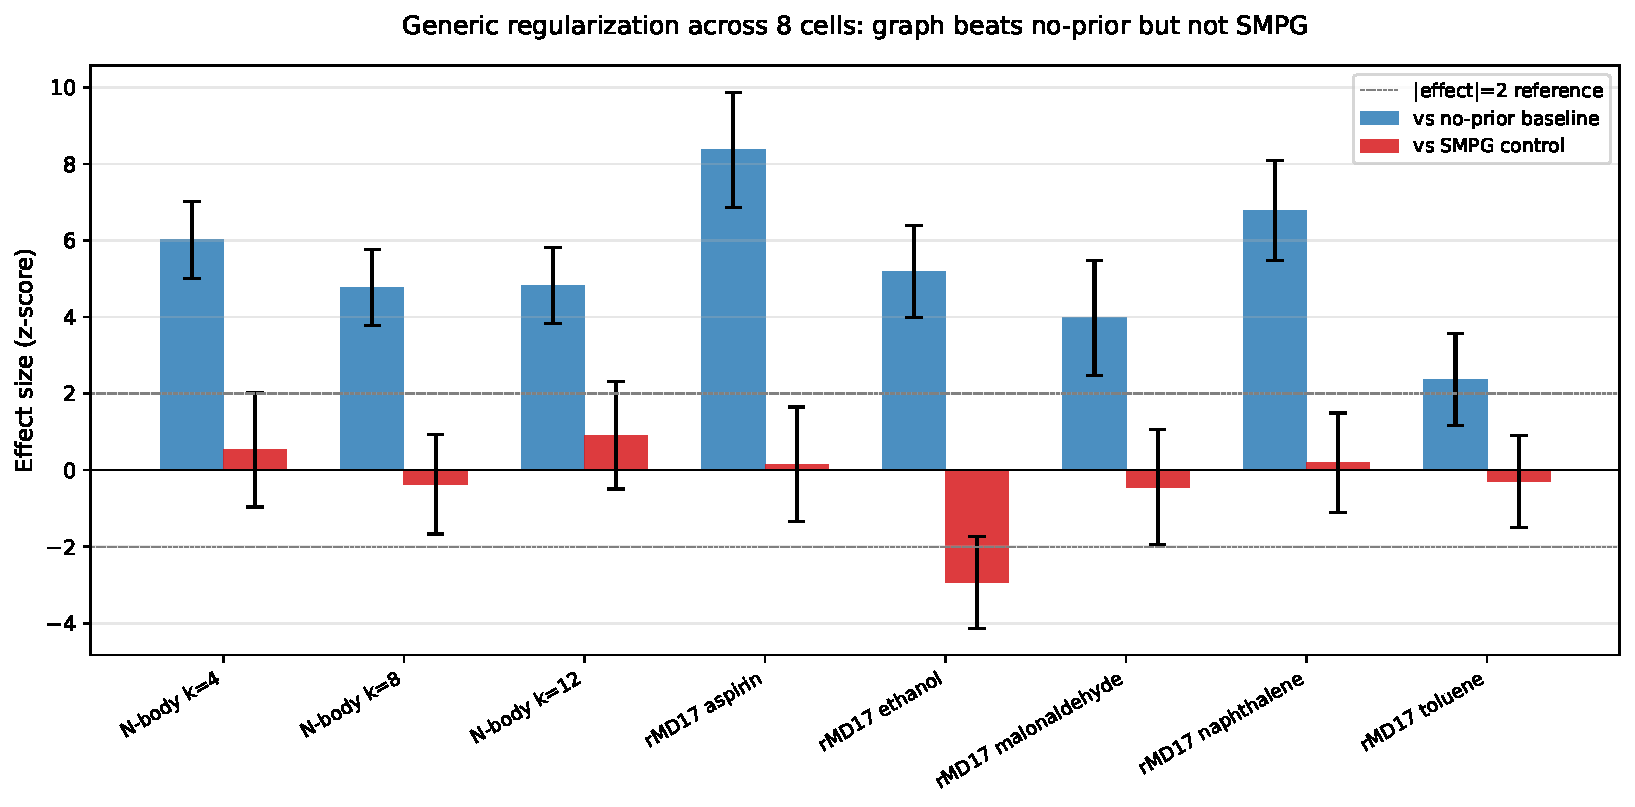
\includegraphics[width=0.95\linewidth]{figures/fig_generic_regularization_8cells.pdf}
\caption{Generic-regularization cells: effect sizes against no-prior 
baseline (left bars) versus against SMPG control (right bars), with 
95\% confidence intervals. In all eight cells the candidate graph 
substantially improves rollout over no-prior training (left bars), 
but the improvement does not separate from the SMPG control (right 
bars) under the operational non-overlapping CI criterion.}
\label{fig:generic-reg}
\end{figure}

\subsection{No-effect cells}
\label{sec:no-effect}

Four cells show no meaningful candidate-graph effect at standard 
budget. Spring-mass lattice has graph H32 = 0.0800 ± 0.0379 versus 
none = 0.0815 ± 0.0136 (effect 0.09, CI overlap). Graph-wave lattice 
has graph 0.0782 ± 0.0324 versus none 0.0833 ± 0.0249 (effect 0.35, 
overlap). METR-LA correlation graph has graph 0.5243 ± 0.2845 versus 
none 0.4034 ± 0.0609 (effect $-0.74$; the candidate graph performs 
worse than no-prior on average, although CIs overlap). Graph-heat 
lattice is retained as a legacy single-seed cautionary cell in the 
no-effect block, although it is not part of the multiseed subset: 
graph H32 = 0.6902 versus none = 0.6036, so the candidate graph 
performs worse under the tested model condition. The protocol's 
output for these cells is "do not carry the candidate graph forward 
in this model condition", which we treat as the appropriate honest 
recommendation.

\subsection{Methodological cross-validation}
\label{sec:cross-val}

As representative methodological cross-checks, we run node-order and 
transition-design diagnostics in selected regimes.

\paragraph{Node-order sanity check.}
In spring-mass and N-body $k$=4, we run a node-order sanity check 
that probes whether the model's prediction pathway is sensitive to 
graph–data alignment. Three conditions are compared: (A) baseline 
(data and graph both unpermuted), (B) data and graph permuted 
consistently with the same permutation (permutation-equivariance 
check), and (C) data permuted while the candidate graph is left 
unchanged (alignment-break stress). In spring-mass, the H32 values 
are A = 0.62 ± 0.17, B = 0.62 ± 0.17, C = 0.74 ± 0.35. The B = A 
equality confirms permutation equivariance; the C value is only 
$\sim 19\%$ worse than A despite breaking graph–data alignment, 
indicating that the prediction pathway weakly utilizes the candidate 
graph in this model condition. A WARNING flag is raised. The same 
WARNING is raised on N-body $k$=4. This independent diagnostic is 
consistent with the generic-regularization classification: the model 
condition does not strongly exploit topology, regardless of prior 
strength.

\paragraph{Transition-architecture redesign.}
\label{sec:transition-control}
As a robustness probe, we also tested whether the 
generic-regularization pattern was an artifact of the pooled-latent 
transition design. Replacing the transition with a graph-aware 
SAGEConv-plus-residual-MLP module stabilized by LayerNorm did not 
rescue topology attribution: spring-mass remained no-effect (effect 
against SMPG = 0.005), and N-body $k$=4 remained generic 
regularization (effect against no-prior = 3.79; effect against SMPG 
= 0.08, CI overlap). The node-order sanity WARNING also persisted. 
We therefore treat generic-regularization dominance as a 
model-condition finding rather than a trivial artifact of the 
original transition head.

\subsection{Summary}
\label{sec:results-summary}

Across 13 measurement cells, the protocol produces three operational 
attribution outputs: one controlled audit-positive / 
topology-aligned support case (HO audit), eight 
generic-regularization cells (three N-body standard cells plus five 
rMD17 molecules), and four no-effect cells. Without SMPG and 
calibrated temporal-smoothing controls, the eight 
generic-regularization cells would have appeared as 
graph-versus-no-prior successes; the protocol redirects this finding 
into the appropriate attribution class. We discuss the implications 
in Section~\ref{sec:discussion}.

\begin{table}[h]
\centering
\scriptsize
\setlength{\tabcolsep}{3pt}
\renewcommand{\arraystretch}{1.08}
\caption{Unified effect-size table. Effect sizes are computed as (comparator\_mean - graph\_mean) / (std\_graph / sqrt(n\_graph)). Positive values indicate the candidate graph achieves lower H32 rollout error. CI overlap labels are based on 95\% confidence intervals.}
\label{tab:effect-size}
\resizebox{\textwidth}{!}{%
\begin{tabular}{llccccccccccc}
\toprule
regime & cell & n\_seeds & mean H32 graph & effect vs none & CI vs none & effect vs SMPG & CI vs SMPG & effect vs random & CI vs random & effect vs temporal & CI vs temporal & classification \\
\midrule
\path{ho_audit_5seed} & \path{ho_lattice_audit} & 5 & $0.0169$ & N/A & N/A & $3.083$ & non-overlap & $2.745$ & non-overlap & N/A & N/A & \texttt{controlled\_audit\_positive} \\
\path{nbody_robustness_5seed} & \path{distance_k_04/standard_ep20} & 5 & $0.0641$ & $6.014$ & non-overlap & $0.535$ & overlap & N/A & N/A & $0.139$ & overlap & \texttt{generic\_regularization} \\
\path{nbody_robustness_5seed} & \path{distance_k_08/standard_ep20} & 5 & $0.0814$ & $4.768$ & non-overlap & $-0.370$ & overlap & N/A & N/A & $-0.801$ & overlap & \texttt{generic\_regularization} \\
\path{nbody_robustness_5seed} & \path{distance_k_12/standard_ep20} & 5 & $0.0772$ & $4.824$ & non-overlap & $0.906$ & overlap & N/A & N/A & $-1.265$ & overlap & \texttt{generic\_regularization} \\
\path{rmd17_cycle2_3seed} & aspirin & 3 & $0.0306$ & $8.367$ & non-overlap & $0.147$ & overlap & $-0.013$ & overlap & N/A & N/A & \texttt{generic\_regularization} \\
\path{rmd17_cycle2_3seed} & ethanol & 3 & $0.0449$ & $5.196$ & overlap & $-2.935$ & overlap & $-2.358$ & overlap & N/A & N/A & \texttt{generic\_regularization} \\
\path{rmd17_cycle2_3seed} & malonaldehyde & 3 & $0.0346$ & $3.979$ & overlap & $-0.445$ & overlap & $-0.480$ & overlap & N/A & N/A & \texttt{generic\_regularization} \\
\path{rmd17_cycle2_3seed} & naphthalene & 3 & $0.0210$ & $6.785$ & non-overlap & $0.191$ & overlap & $0.381$ & overlap & N/A & N/A & \texttt{generic\_regularization} \\
\path{rmd17_cycle2_3seed} & toluene & 3 & $0.0323$ & $2.359$ & overlap & $-0.289$ & overlap & $-0.247$ & overlap & N/A & N/A & \texttt{generic\_regularization} \\
\path{graph_heat_lattice} & \path{legacy_ep5_no_quick_tag} & 1 & $0.6902$ & N/A & non-overlap & N/A & non-overlap & N/A & N/A & N/A & N/A & \texttt{no\_effect} \\
\path{graph_wave_5seed} & \path{standard_ep20} & 5 & $0.0782$ & $0.352$ & overlap & $-0.469$ & overlap & N/A & N/A & $-0.559$ & overlap & \texttt{no\_effect} \\
\path{metr_la_3seed} & \path{corr_T2000_train160_ep5} & 3 & $0.5243$ & $-0.736$ & overlap & $-0.132$ & overlap & N/A & N/A & $-0.089$ & overlap & \texttt{no\_effect} \\
\path{spring_mass_5seed} & \path{standard_ep20} & 5 & $0.0800$ & $0.088$ & overlap & $0.189$ & overlap & N/A & N/A & $-0.024$ & overlap & \texttt{no\_effect} \\
\bottomrule
\end{tabular}
}
\noindent\emph{Note.} HO audit graph-vs-control effects use paired bootstrap deltas from the specificity audit because the audit cell has no no-prior arm. \texttt{controlled\_audit\_positive} denotes the controlled audit-positive class; HO audit is the only such case in our evidence.
\end{table}

\FloatBarrier

\section{Discussion}
\label{sec:discussion}

The main contribution of the manuscript is methodological. It 
provides a principled way to decide, under a fixed model condition, 
whether a graph-prior gain supports candidate topology, generic 
regularization, or no meaningful graph effect. In that sense, the 
protocol addresses a recurring problem in computational science: 
prior choice is consequential, but prior interpretation is easy to 
overstate.

The reported cases sharpen the distinction between predictive 
utility and topology-specific attribution. A candidate graph 
beating the no-prior baseline can be useful, but it has not yet 
shown that node-label structure matters. Across 13 measurement 
cells, the protocol assigns one cell to controlled audit-positive / 
topology-aligned support (HO lattice audit), eight cells to generic 
regularization (three N-body standard cells and five rMD17 
molecules), and four cells to no-effect. The dominant pattern is 
generic regularization rather than topology-aligned support: in 
the eight generic-regularization cells, effect sizes against the 
no-prior baseline range from 2.4 to 8.4, but effect sizes against 
the SMPG control range from $-2.9$ to 0.9 with confidence-interval 
overlap in every cell. Without SMPG controls, these eight cells 
would have been over-attributed as graph-versus-no-prior successes; 
the protocol redirects them into the appropriate attribution class.

Several model-condition observations emerge from this evidence. 
First, the prediction pathway in our tested architecture weakly 
exploits topology even when the candidate graph is structurally 
plausible. The node-order sanity check provides an independent 
diagnostic of this insensitivity: in spring-mass, the alignment-break 
stress is only \(\sim 19\%\) worse than baseline, and N-body \(k=4\) 
produces the same warning-level diagnostic. Second, the 
generic-regularization classification is not a trivial artifact of 
the pooled-latent transition design: replacing the transition with a 
graph-aware SAGEConv-plus-residual-MLP module did not rescue topology 
attribution. We therefore treat generic-regularization dominance as 
a model-condition finding rather than a purely architectural failure.

The HO audit deserves special discussion. It is the only cell in 
our evidence where rollout point-estimate ordering and audit-mode 
latent metrics agree in the direction predicted by topology-aligned 
learning. Importantly, even here the rollout confidence intervals 
overlap; the audit-positive classification rests on the agreement 
between rollout ordering and latent-space audit metrics rather than 
on rollout CI separation. This is a deliberately conservative 
operational standard. The HO setting is also the only cell where 
the candidate graph corresponds exactly to the physical Laplacian, 
making it a controlled best case rather than a topology-discovery 
result.

The negative cases reinforce the same operational lesson. METR-LA 
diagnoses candidate-graph construction risk: the tested 
correlation-derived graph fails without ruling out official road 
adjacency, road-distance graphs, or learned traffic graphs. Graph 
heat diagnoses prior-form risk: even a true generator graph can fail 
when static Laplacian smoothing is mismatched to diffusion-like 
transition dynamics. Spring-mass and graph-wave show how the same 
workflow can recommend against carrying a candidate graph forward 
when it fails to clear the baseline. The value of the protocol, 
therefore, lies as much in ruling out unsupported interpretations as 
in identifying promising priors.

The practical value is attribution control: the protocol turns 
graph-prior successes, failures, and heterogeneous outcomes into 
diagnostic categories with explicit claim boundaries. 
Table~\ref{tab:claims-evidence} summarizes the principal claims, 
their evidentiary basis, and the boundaries that accompany them. 
Detailed case-level traceability is retained in 
Appendix~\ref{app:traceability}.

\begingroup
\scriptsize
\setlength{\tabcolsep}{3pt}
\renewcommand{\arraystretch}{1.08}
\begin{longtable}{>{\raggedright\arraybackslash}p{0.22\textwidth}>{\raggedright\arraybackslash}p{0.18\textwidth}>{\raggedright\arraybackslash}p{0.31\textwidth}>{\raggedright\arraybackslash}p{0.21\textwidth}}
\caption{Claims, evidence, and boundaries}\label{tab:claims-evidence}\\
\toprule
\textbf{manuscript claim} & \textbf{supporting evidence} & \textbf{key numbers} & \textbf{boundary} \\
\midrule
\endfirsthead
\toprule
\textbf{manuscript claim} & \textbf{supporting evidence} & \textbf{key numbers} & \textbf{boundary} \\
\midrule
\endhead
\midrule
\multicolumn{4}{r}{\emph{Continued on next page}} \\
\midrule
\endfoot
\bottomrule
\endlastfoot
The preflight protocol gives actionable prior recommendations. & Preflight benchmark summary and individual preflight reports. & Operational attribution labels include no gain, temporal sufficient, candidate topology-specific, generic smoothing, and audit-supported positive cases. & Recommendations apply only under tested model and budget conditions. \\
In this protocol, the spectrum-matched permuted graph control is necessary for topology-specific attribution. & Master decision rules and graph specificity table. & HO lattice lambda=0.1 beats the spectrum-matched permuted graph control at H32; many rMD17 cases do not. & In our evidence, a candidate graph beating no-prior training alone would have been over-attributed without SMPG controls. \\
Calibrated temporal smoothing changes candidate graph attribution. & Calibrated spring-mass, graph-wave, and n-body preflight reports. & Spring-mass temporal H32 $0.5689$ vs graph $0.5740$; graph-wave temporal H32 $0.5663$ vs graph $0.5712$; n-body graph H32 $0.5433$ vs temporal $0.6453$. & Calibration is required because raw prior losses differ by scale. \\
Candidate-graph gains can be low-budget-only. & Quick/standard comparisons for spring-mass, graph-wave, and n-body. & Spring-mass graph H32 quick $0.5740$ vs standard $0.1048$, while standard no-prior is $0.0809$; graph-wave standard no-prior is best; n-body standard spectrum-matched permuted graph control is best. & This does not imply that graph priors never help longer runs. \\
N-body standard cells show generic regularization, not topology-specific attribution. & N-body standard calibrated preflight reports. & H32 ($k=4$ standard, 5 seeds) none $0.151 \pm 0.013$, graph $0.064 \pm 0.032$, permuted $0.072 \pm 0.025$, temporal $0.066 \pm 0.015$. Effect vs none 6.01 (non-overlap); effect vs SMPG 0.54 (overlap); effect vs temporal 0.14 (overlap). & Pattern persists at $k=8,12$. SMPG and temporal controls explain the apparent gain. \\
Audit mode can support topology-aligned latent smoothing. & Cycle 8 checkpointed HO lattice audit. & H32 graph $0.0169$, permuted control $0.0198$, random $0.0199$; graph $D_{\mathrm{true},\mathrm{norm}}(\Delta H)$ $2.8106$ vs permuted control $3.5109$; graph $R_{\mathrm{low}}$ at $K=4$ $0.1866$ vs $0.1216$. & This is a controlled audit-positive case, not universal latent-alignment evidence. \\
Raw graph-dynamics alignment is not sufficient. & Cycle 6 diagnostics, METR-LA, graph low-frequency lattice, graph heat. & METR raw true $D_{dX,\mathrm{norm}}$ $0.2380$ vs permuted $0.3044$, but graph H32 is worse than no-prior training; the graph low-frequency case also fails to establish quick topology-specific attribution. & Raw diagnostics are supporting probes, not decision rules. \\
Graph-generated dynamics do not guarantee candidate graph utility. & Graph heat lattice report and failure audit. & H32 none $0.6036$, graph $0.6902$, permuted control $0.6058$. & The prior acts on learned latents, not directly on the simulator equation. \\
\end{longtable}
\endgroup

\FloatBarrier

\section{Limitations}

The protocol is intentionally conservative. Its recommendations are model-conditioned and budget-conditioned: they apply to the tested encoder, transition model, latent dimension, prior placement, optimizer settings, prior strength, training budget, and rollout horizon. A recommendation should therefore be treated as a local computational conclusion rather than as a property of the dataset alone.

Several methodological boundaries follow from this framing. Candidate graphs in the reported regimes range from simulator-defined lattices to approximate physical constructions and data-derived correlation graphs, and those categories should not be interpreted in the same way. The spectrum-matched permuted graph control is the strongest control used here, but it does not exhaust every possible graph confound. Calibrated temporal smoothing is required for fair graph-versus-temporal comparison. Raw-coordinate diagnostics such as $D_L(\\Delta X)$ can be useful supporting probes, but because the prior acts on learned latents, they are not sufficient decision rules.

A further limitation is that audit mode depends on checkpointed latent traces or saved latent artifacts. Where those artifacts are missing, mechanism claims must remain limited. Finally, the benchmark spans representative node-wise physical/scientific dynamics regimes rather than the whole space of scientific prediction problems. The manuscript should therefore not be read as introducing a universal physics predictor, a causal discovery method, or a state-of-the-art benchmark.

Table 5 consolidates these boundaries in the form used throughout the draft.

\begingroup
\footnotesize
\setlength{\tabcolsep}{4pt}
\begin{longtable}{>{\raggedright\arraybackslash}p{0.18\textwidth}>{\raggedright\arraybackslash}p{0.44\textwidth}>{\raggedright\arraybackslash}p{0.28\textwidth}}
\caption{Limitations and claim boundaries}\label{tab:limitations-boundaries}\\
\toprule
\textbf{limitation or boundary} & \textbf{boundary statement} & \textbf{implication} \\
\midrule
\endfirsthead
\toprule
\textbf{limitation or boundary} & \textbf{boundary statement} & \textbf{implication} \\
\midrule
\endhead
\midrule
\multicolumn{3}{r}{\emph{Continued on next page}} \\
\midrule
\endfoot
\bottomrule
\endlastfoot
Model conditioning & Recommendations apply under the tested encoder, transition model, prior placement, prior strength, optimizer, training budget, and rollout horizon. & Changing the model condition requires a new preflight interpretation. \\
Budget conditioning & Quick-mode gains can disappear under standard or longer training. & Quick positives should be validated before stronger claims. \\
Candidate graph ambiguity & Candidate graphs may be true, approximate, constructed, or data-derived. & A useful candidate graph prior does not prove physical truth. \\
Control requirements & In this protocol, topology-specific attribution requires beating the spectrum-matched permuted graph control and calibrated temporal smoothing. & Graph versus none is insufficient for topology-specific attribution. \\
Temporal calibration & Raw temporal prior losses may be much smaller than graph-prior losses. & Temporal baselines should be calibrated before attribution. \\
Raw diagnostics & Raw-coordinate smoothness can disagree with learned latent prior utility. & Raw $D_L(\Delta X)$ should not be used as a sufficient decision rule. \\
Audit artifacts & Latent audits require saved traces or checkpoints. & Missing artifacts limit mechanism claims. \\
Benchmark scope & Regimes are representative stress tests, not universal physics coverage. & Avoid universal predictor or SOTA benchmark framing. \\
Causal claims & The workflow compares predictive priors and controls. & Do not frame the result as causal discovery. \\
Prior novelty & The graph Laplacian prior is a tested prior family, not the paper's algorithmic novelty. & The contribution is the preflight protocol and attribution workflow. \\
\end{longtable}
\endgroup

\section{Conclusion}
\label{sec:conclusion}

This manuscript presents a model-conditioned preflight protocol for 
prior selection in node-wise scientific latent dynamics. By combining 
no-prior baselines, a candidate graph prior, the spectrum-matched 
permuted graph control, calibrated temporal smoothing, and audit 
mode when latent artifacts are available, the protocol turns prior 
choice into a structured computational decision rather than an ad 
hoc modeling preference.

Across 13 measurement cells in seven regimes, the dominant pattern 
is generic regularization rather than topology-aligned support. 
Eight of the 13 cells, spanning N-body synthetic data and five 
rMD17 molecules, show that graph priors substantially improve 
prediction over no-prior training but do not separate from the 
spectrum-matched permuted graph control under the operational 
non-overlapping confidence-interval criterion. The HO lattice 
audit is the single controlled audit-positive / topology-aligned 
support case, where rollout ordering and audit-mode latent metrics 
agree in the direction predicted by topology-aligned learning. Four 
no-effect cells (spring-mass, graph-wave, METR-LA, graph-heat) show 
that graph priors do not always provide regularization benefit even 
under matched conditions. In our evidence, graph-versus-no-prior 
improvements would have been over-attributed without SMPG controls.

The contribution is therefore a practical workflow for prior 
selection and interpretation rather than a new graph prior, a 
universal physics predictor, a causal discovery method, or a 
state-of-the-art benchmark. The protocol's primary value is 
attribution control: it converts ambiguous "graph-vs-none" gains 
into structured operational classes that can guide subsequent 
computational decisions under a fixed model condition.

\section*{Data and Code Availability}
This manuscript reports previously completed runs only and introduces no new experiments in this version. The preflight tool is implemented in the project repository as an adapter-based script in which dataset-specific adapters provide trajectories and candidate graph information, while the shared routine writes \texttt{run\_config.json}, \texttt{summary.csv}, and \texttt{preflight\_report.md} as standardized run artifacts. Code and manuscript assets are available at \url{https://github.com/2GyounnnG/causalworld}. A versioned archival snapshot will be provided upon publication or repository release.

\FloatBarrier

\appendix

\section{Protocol details and operating modes}

The protocol is best understood as a sequence of increasingly demanding questions. The first question is whether any prior helps over no-prior training. The second is whether the gain survives the spectrum-matched permuted graph (SMPG) control and calibrated temporal smoothing. Audit mode, when checkpointed latent traces are available, asks whether predictive gains coincide with latent behavior consistent with the candidate graph. The strongest label therefore requires agreement across utility, control comparisons, and latent-space evidence.

The labels in Table 1 should be interpreted as report-level decisions rather than as permanent properties of a dataset. They are intentionally conservative: \path{no_prior_gain} and \path{overconstrained} recommend against continuing the prior; \path{temporal_smoothing_sufficient} recommends a cheaper graph-free alternative; \path{candidate_topology_specific} supports topology-specific attribution under the tested condition; and \path{topology_aligned_latent_smoothing} requires audit evidence in addition to predictive gains.

\section{Benchmark regimes and dataset-adapter notes}

The benchmark set mixes graphs with different provenance. HO, spring-mass, graph-wave, and graph heat use true or simulator-defined lattices. The graph low-frequency regime uses a constructed spectral stress test. N-body uses an approximate distance-kNN graph. The rMD17 summaries use molecular cutoff graphs. METR-LA uses a correlation-derived sensor graph. This variation is intentional because candidate graph provenance is part of the interpretation boundary addressed by the preflight protocol.

\section{Prior families and calibration formulas}

The graph Laplacian prior on learned node-wise latent states is

\begin{equation}
R_G(H;L)=\mathrm{Tr}(H^\top L H)
\end{equation}

The spectrum-matched permuted graph control is

\begin{equation}
L_{\mathrm{perm}} = P^T L P,
\end{equation}

where $P$ is a permutation matrix. This preserves Laplacian eigenvalues while disrupting node-label semantics.

The graph-free temporal smoothness prior is

\begin{equation}
R_T(H_{1:T})=\sum_t \lVert H_{t+1}-H_t \rVert_F^2
\end{equation}

For calibrated prior-strength matching, let $\alpha_G$ be the graph-prior weight, and let $R_G^0$ and $R_T^0$ denote initial graph and temporal prior losses under the same calibration pass. The calibrated temporal weight is

\begin{equation}
\alpha_T = \frac{\alpha_G R_G^0}{R_T^0+\varepsilon}
\end{equation}

so that

\begin{equation}
\alpha_T R_T^0 \approx \alpha_G R_G^0
\end{equation}

\section{Claim traceability and supporting evidence}
\label{app:traceability}

This appendix provides a compact traceability table linking each major manuscript claim to the supporting experiment summaries, key numerical evidence, and interpretation caveats.

\begingroup
\scriptsize
\setlength{\tabcolsep}{3pt}
\begin{longtable}{>{\raggedright\arraybackslash}p{0.22\textwidth}>{\raggedright\arraybackslash}p{0.18\textwidth}>{\raggedright\arraybackslash}p{0.21\textwidth}>{\raggedright\arraybackslash}p{0.17\textwidth}>{\raggedright\arraybackslash}p{0.12\textwidth}}
\caption{Claim traceability and supporting evidence}\label{tab:evidence-map}\\
\toprule
\textbf{claim} & \textbf{supporting evidence} & \textbf{key numbers} & \textbf{caveats} & \textbf{appears in} \\
\midrule
\endfirsthead
\toprule
\textbf{claim} & \textbf{supporting evidence} & \textbf{key numbers} & \textbf{caveats} & \textbf{appears in} \\
\midrule
\endhead
\midrule
\multicolumn{5}{r}{\emph{Continued on next page}} \\
\midrule
\endfoot
\bottomrule
\endlastfoot
The paper contributes a computational preflight protocol for model-conditioned prior selection. & \path{paper/jcs_outline.md}; \path{paper/jcs_draft_intro.md}; \path{paper/jcs_draft_methods.md} & Model condition includes encoder, transition model, prior placement, strength, training budget, and rollout horizon. & Not a new graph prior or SOTA benchmark. & Tables 1-2 \\
In this protocol, the spectrum-matched permuted graph control is the key topology-specific attribution control. & \path{paper/jcs_draft_methods.md}; \path{paper/tables/evidence_map.md} & $L_{\mathrm{perm}} = P^\top L P$; HO lattice lambda=0.1 permuted-control delta $0.002866$ at H32 with CI $[0.001070, 0.004210]$. & Random graph controls are secondary and not fully spectrum-matched. & Tables 2 and 4 \\
Calibrated temporal smoothing can explain some candidate graph gains. & \path{paper/tables/evidence_map.md}; \path{paper/tables/table4_claims_evidence.md} & Spring-mass temporal H32 $0.5689$ vs graph $0.5740$; graph-wave temporal H32 $0.5663$ vs graph $0.5712$. & Requires calibrated prior strength; uncalibrated temporal comparisons are not enough. & Tables 1 and 4 \\
N-body standard cells show generic regularization, not topology-specific attribution. & \path{paper/tables/evidence_map.md}; \path{paper/tables/table4_claims_evidence.md} & H32 ($k=4$ standard, 5 seeds) none $0.151 \pm 0.013$, graph $0.064 \pm 0.032$, permuted $0.072 \pm 0.025$, temporal $0.066 \pm 0.015$. Effect vs none 6.01 (non-overlap); effect vs SMPG 0.54 (overlap); effect vs temporal 0.14 (overlap). & Pattern persists at $k=8,12$. SMPG and temporal controls explain the apparent gain. & Section 7; Tables 3-4 \\
HO lattice/Cycle 8 is a controlled audit-positive / topology-aligned support case. & \path{paper/tables/evidence_map.md}; \path{paper/figure_data/fig6_latent_audit_positive_case.csv} & H32 graph $0.0169$, permuted $0.0198$, random $0.0199$; $D_{\mathrm{true},\mathrm{norm}}(\Delta H)$ graph $2.8106$, permuted $3.5109$, random $3.5237$; $R_{\mathrm{low}}$ true $K=4$ graph $0.1866$, permuted $0.1216$. & Rollout CIs overlap across arms; classification rests on agreement between rollout point-estimate ordering and audit metrics. Controlled best case; not a topology-discovery result. & Figure 3; Tables 3-4 \\
METR-LA correlation graph demonstrates no graph gain despite raw alignment. & \path{paper/tables/evidence_map.md}; \path{paper/tables/table4_claims_evidence.md} & Raw true $D_{dX,\mathrm{norm}}$ $0.2380$, permuted $0.3044$, random $0.4737$; H32 none $0.4068$, graph $0.4461$, permuted $0.4337$. & Uses \texttt{correlation\_topk} graph, not official road adjacency. & Tables 3-5 \\
Graph heat lattice shows true generator graph does not guarantee prior utility. & \path{paper/tables/evidence_map.md}; \path{paper/tables/table4_claims_evidence.md} & H32 none $0.6036$, graph $0.6902$, permuted $0.6058$. & Applies to the tested latent model and prior setting. & Tables 3-5 \\
rMD17 5-molecule Cycle-2 evidence corroborates the generic-regularization classification on real molecular dynamics. & \path{paper/tables/evidence_map.md}; \path{paper/tables/table4_claims_evidence.md} & 5/5 molecules: graph reduces H32 vs \texttt{gnn\_node} none (effect sizes 2.36-8.37). 0/5 molecules show non-overlapping CI vs SMPG control. 3/5 molecules: SMPG or random matches/outperforms graph. & 3-seed Cycle-2 historical data; no calibrated temporal-smoothing arm, so used as corroborating cross-domain evidence. & Tables 3-4 and discussion \\
\end{longtable}
\endgroup

\section{Reproducibility note and software interface}

The present draft summarizes previously completed runs only. The software interface follows an adapter-based design in which dataset-specific trajectory loading and candidate graph Laplacian construction or loading are handled by adapters, while the core routine carries out the matched prior comparisons under a shared model condition. In this interface, \path{run_config.json} records the run specification, \path{summary.csv} provides the compact metric summary, and \path{preflight_report.md} provides the human-readable report and actionable prior recommendation. Companion documentation targets for this tool include \path{paper/tool_readme_draft.md} and \path{docs/graph_prior_preflight_tool.md}, alongside the command-line example below.

\begingroup
\footnotesize
\begin{verbatim}
conda run -n causalworld python scripts/graph_prior_preflight_check.py \
  --dataset spring_mass_lattice \
  --prior-weight 0.1 \
  --epochs 5 \
  --train-transitions 96 \
  --eval-transitions 32 \
  --horizons 16 32 \
  --include-temporal-prior \
  --calibrate-prior-strength \
  --out-dir analysis_out/preflight_runs/spring_mass_lattice_ep5_temporal_calibrated
\end{verbatim}
\endgroup

This command is included for interface clarity only; no new experiment is introduced in this manuscript version.

\bibliographystyle{elsarticle-num}
\IfFileExists{paper/references.bib}{\bibliography{paper/references}}{\bibliography{references}}

\end{document}
